%  article.tex (Version 3.3, released 19 January 2008)
%  Article to demonstrate format for SPIE Proceedings
%  Special instructions are included in this file after the
%  symbol %>>>>
%  Numerous commands are commented out, but included to show how
%  to effect various options, e.g., to print page numbers, etc.
%  This LaTeX source file is composed for LaTeX2e.

%  The following commands have been added in the SPIE class
%  file (spie.cls) and will not be understood in other classes:
%  \supit{}, \authorinfo{}, \skiplinehalf, \keywords{}
%  The bibliography style file is called spiebib.bst,
%  which replaces the standard style unstr.bst.
\RequirePackage{snapshot}
\newcommand{\argmin}[1]{\underset{#1}{\operatorname{arg}\,\operatorname{min}}\;}

\documentclass[12pt]{spieman}
%%\documentclass[letter]{spie}  %>>> use for US letter paper
%%\documentclass[a4paper]{spie}  %>>> use this instead for A4 paper
%%\documentclass[nocompress]{spie}  %>>> to avoid compression of citations
%% \addtolength{\voffset}{9mm}   %>>> moves text field down
%\renewcommand{\baselinestretch}{1.65}   %>>> 1.65 for double spacing, 1.25 for 1.5 spacing


\makeatletter
\@fpsep\textheight
\makeatother


%% Latex documents that need direct input
\title{Non Destructive Testing based on a Scanning-From-Heating approach: Application to non-through defect detection and fiber orientation assessment}

\author[a]{Belkacemi M.}
\author[a]{Stolz C.}
\author[b]{Mathieu A.}
\author[a,c]{Lemaitre G.}
\author[a]{Massich J.}
\author[a]{Aubreton O.}
\affil[a]{LE2I UMR6306, CNRS, Arts et M\'etiers, Univ. Bourgogne Franche-Comt\'e, 12 rue de la Fonderie, Le Creusot, France, 71200}
\affil[b]{ICB, UMR 6303 CNRS-Universit\'e Bourgogne Franche-Comt\'e, 12 rue de la Fonderie, Le Creusot, France, 71200}
\affil[c]{ViCOROB, Universitat de Girona, Campus Montilivi, Edifici P4, Girona, Spain, 17071}




%  The following command loads a graphics package to include images
%  in the document. It may be necessary to specify a DVI driver option,
%  e.g., [dvips], but that may be inappropriate for some LaTeX
%  installations.
\usepackage{subfigure}
\usepackage[]{graphicx}

% In order to include files without having a clear page using \include*,
% the newclude package is required
\usepackage{newclude}

% Required for acronyms
% use \acresetall to reset the acroyms counter
% macros=True, allows for calling \myTriger rather than \ac{myTriger}
\usepackage[single=true, macros=true, xspace=true]{acro}

% In SPIE template, biblatex can NOT be used to manage the referencing
%
%\usepackage[style=spiebib, backend=biber]{biblatex}

% Clever cross referencing. Using cleverref, instead of writting
% figure~\ref{...} or equation~\ref{...}, only \cref{...} is required.
% The package interprates the references and introduces the figure, fig.,
% equation, eq., etc keywords. \Cref forces first letter capital.
% >> WARNING: This package needs to be loaded after hyperref, math packages,
%             etc. if used.
%             Cleveref is recomended to load late
\usepackage{hyperref}
\usepackage{cleveref}

% To create random text use lipsum
\usepackage{lipsum}

% math package
\usepackage{amsmath,amsfonts, amssymb}

% units package
\usepackage{siunitx}
%array
\usepackage{multirow}

% acronym
\usepackage{acro}

% Include the following packages to use tikz
\usepackage{tikz,xifthen}
\usepackage{tikz-qtree}
\usetikzlibrary{decorations.pathmorphing} % noisy shapes
\usetikzlibrary{fit}% fitting shapes to coordinates
\usetikzlibrary{backgrounds}% drawing the background after the foreground
\usetikzlibrary{shapes,arrows,shadows}
\usetikzlibrary{calc,decorations.pathreplacing,decorations.markings,positioning}
\usetikzlibrary{snakes,decorations.text,shapes,patterns}
\usepackage{transparent}

\usepackage[skins]{tcolorbox}

%% Acronym definition example using glossaries package
%% \usepackage{acro} is required
%% 
%% For a powerful usage of the acro package look at http://tex.stackexchange.com/questions/135975/how-to-define-an-acronym-by-using-other-acronym-and-print-the-abbreviations-toge

\DeclareAcronym{ndt}{
  short = NDT ,
  long = Non-Destructive Testing
}

\DeclareAcronym{sfh}{
  short = SFH,
  long = Scanning-From-Heating
}

\DeclareAcronym{pt}{
  short = PT,
  long = Pulse Thermography
}

\DeclareAcronym{ppt}{
  short = PPT,
  long = Pulse Phase Thermography
}

\DeclareAcronym{lt}{
  short = LT,
  long = Lock-in Thermography
}

\DeclareAcronym{fem}{
  short = FEM,
  long = Finite Element Method
}

\DeclareAcronym{sthm}{
  short = SThM,
  long = Thermal Scanning Microscope
}

\DeclareAcronym{sem}{
  short = SEM,
  long = Scanning Electron Microscope
}

\DeclareAcronym{roi}{
  short = ROI,
  long = Region Of Interest
}

%% Select inputing only one part of the document
%\includeonly{content/intro/intro}   % the file wihtout .tex
%\includeonly{content/other/other_content}

% \addbibresource{./content/lit_review.bib}
% \addbibresource{./content/biblatex-examples.bib}

\begin{document}

\maketitle

\begin{abstract}
\acresetall  % reset the acronyms from the title (if any)
Nowadays, industries ensure the quality of their manufactured products through computer vision techniques and non-conventional imaging. 3D scanners and \ac{ndt} systems are commonly used independently for such applications. Furthermore, these approaches combined together constitute a hybrid systems providing a 3D reconstruction and \ac{ndt} analysis. These systems, however, suffer from drawback such as errors during the data fusion and higher cost for manufacturers. In an attempt to solve those problems, a single active thermography system based on \ac{sfh} is proposed in this paper. Besides 3D digitization of the object, our contributions are twofold: (i) the non-through defect detection for homogeneous metallic object and (ii) fiber orientation assessment for long fiber composite material. The experiments on steel and aluminum plates show that our method achieves to detect non-through defects. Additionally, the estimation of the fiber orientation is evaluated on carbon-fiber composite material.
\end{abstract}

\keywords{Non Destructive Testing, Active Thermography, 3D scanning, Fiber orientation, Non-through defect detection}


%>>>> Include contact information for corresponding author
{\noindent \footnotesize\textbf{*} Mohamed Belkacemi, \linkable{Mohamed.Belkacemi@u-bourgogne.fr} }

%%%%%%%%%%%%%%%%%%%%%%%%%%%%%%%%%%%%%%%%%%%%%%%%%%%%%%%%%%%%%

\begin{spacing}{2}   % use double spacing for rest of manuscript

%%%%%%%%%%%%%%%%%%%%%%%%%%%%%%%%%%%%%%%%%%%%%%%%%%%%%%%%%%%%%

%% Incldue the content without .tex extension
\acresetall  % reset the acronyms from the abstract

% \include*{content/intro/intro}          % the file wihtout .tex
\section{Introduction}

Active infrared thermography becomes one of the essential techniques for \ac{ndt}. Approaches like \ac{pt}\cite{Maldague2002} \ac{ppt} \cite{Maldague1996} or \ac{lt} \cite{Wu1998} have proved to be effective to characterize defects. 
In recent years, an evolution of NDT systems by adding 3D measurement can be noted. Fernandes et al.\cite{fernandes2015fiber} reconstruct carbon fiber objects using 3D scanner and determine the orientation of the fiber with a laser and an infrared camera. Subsequently, the thermal information is mapped to the reconstructed 3D model. Similarly, Oswald-Tranta et al.\cite{Oswald-Tranta2012} detect crack in non-magnetic materials based on the fusion between the infrared and the 3D data, obtained through an inductive \ac{ndt} system and a conventional stereo vision system, respectively.
To quantify the energy losses in buildings, Vidas et al.\cite{Vidas2013} map the thermal information on the 3D data using a Microsoft Kinect and a thermal camera. To conclude, it can be noted that most of the proposed prototypes are actually using two systems: a 3D scanner and a non-destructive inspection system in the infrared range. These hybrid systems in which distinct steps of 3D reconstruction and \ac{ndt} inspection suffer from drawback such as errors during the data fusion.


	%
\begin{figure}
  \centering
  \hspace*{\fill}
  \subfigure[]{\label{subfig:1a}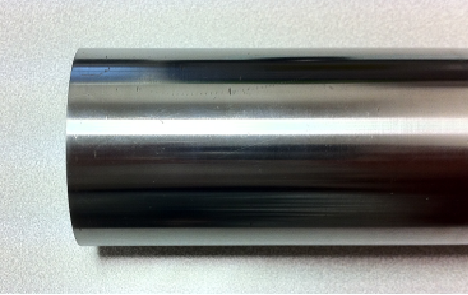
\includegraphics[width=0.15\linewidth]{./Figure/Figure1/A1.png}} \hfill
  \subfigure[]{\label{subfig:1b}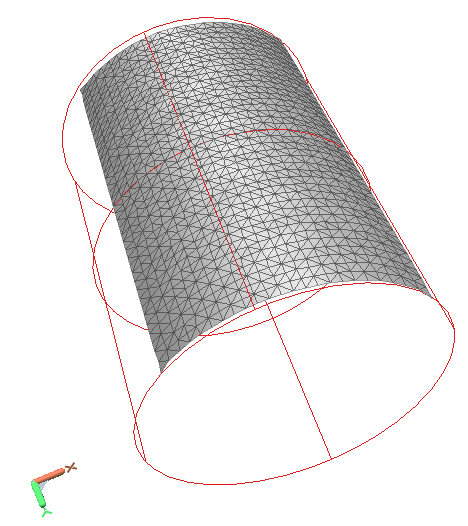
\includegraphics[width=0.15\linewidth]{./Figure/Figure1/A2.png}} \hfill
  \subfigure[]{\label{subfig:1c}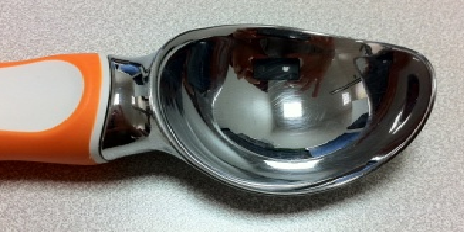
\includegraphics[width=0.15\linewidth]{./Figure/Figure1/B1.png}} \hfill
  \subfigure[]{\label{subfig:1d}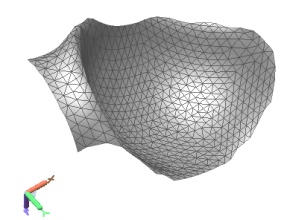
\includegraphics[width=0.15\linewidth]{./Figure/Figure1/B2.png}}
  \hspace*{\fill} \\ \hspace*{\fill}
  \subfigure[]{\label{subfig:1e}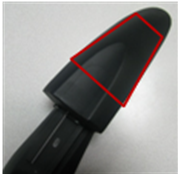
\includegraphics[width=0.15\linewidth]{./Figure/Figure1/C1.png}} \hfill
  \subfigure[]{\label{subfig:1f}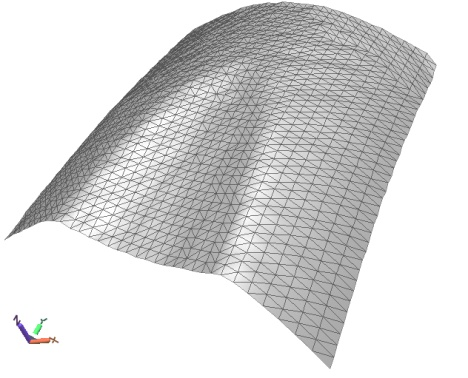
\includegraphics[width=0.15\linewidth]{./Figure/Figure1/C2.png}} \hfill
  \subfigure[]{\label{subfig:1g}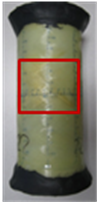
\includegraphics[width=0.1\linewidth]{./Figure/Figure1/D1.png}} \hfill
  \subfigure[]{\label{subfig:1h}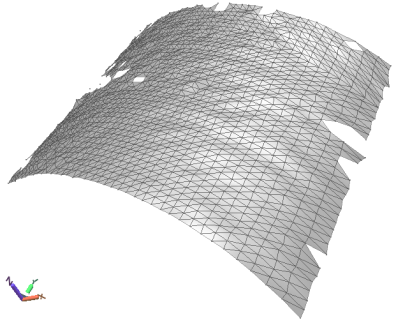
\includegraphics[width=0.15\linewidth]{./Figure/Figure1/D2.png}}
  \hspace*{\fill} \\ \hspace*{\fill}
  \subfigure[]{\label{subfig:1i}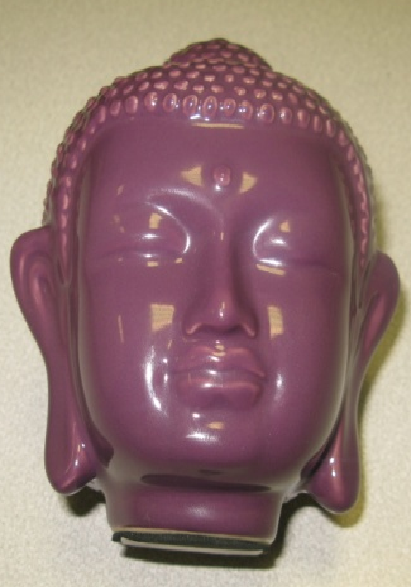
\includegraphics[width=0.15\linewidth]{./Figure/Figure1/E1.png}} \hfill
  \subfigure[]{\label{subfig:1j}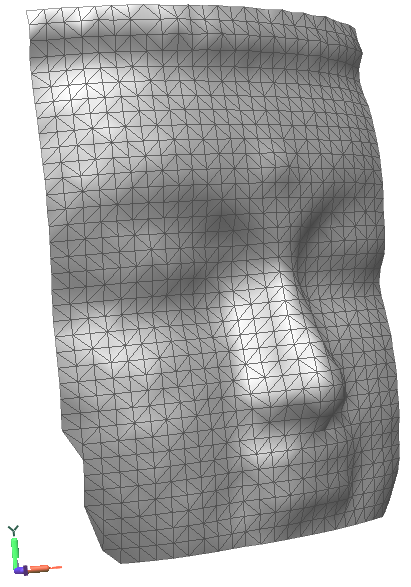
\includegraphics[width=0.15\linewidth]{./Figure/Figure1/E2.png}} \hfill
  \subfigure[]{\label{subfig:1k}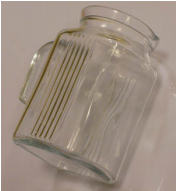
\includegraphics[width=0.15\linewidth]{./Figure/Figure1/F1.png}} \hfill
  \subfigure[]{\label{subfig:1l}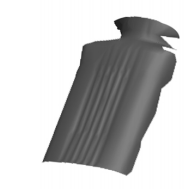
\includegraphics[width=0.15\linewidth]{./Figure/Figure1/F2.png}}
  \hspace*{\fill}
	  \caption{Examples of 3D digitization obtained by \acs*{sfh} approach: (a), (b), (c) and (d) metallic specular surfaces \cite{bajard2013numerisation} - (e) and (f) black plastic - (g) and (h) composite material - (i) and (j) ceramic - (k) and (l) glass transparent object \cite{meriaudeau20113d}.}
  \label{fig:1}
\end{figure}


\ac{sfh} offers an alternative. This approach is initially used to reconstruct objects into 3D. Indeed, Eren et al.\cite{Eren2009} achieve impressive results using \ac{sfh} in which the geometry of glass or plastic transparent objects is estimated based on active triangulation. The transparent object placed on a gliding stage is locally heated using a CO2 laser source of \SI{10.6}{\micro \metre} wavelength. The emitted radiation is acquired by an Infra-Red (IR) camera and the 3D position of the heated point is recovered thanks to a prior calibration, with an accuracy in the order of \SI{100}{\micro \metre}.

Bajard et al.\cite{Bajard2012} have extended this method for metal objects which have different radiative and conductive properties. The CO2 laser source is replaced by an Nd~:YAG Laser of \SI{1.06}{\micro \metre} wavelength, since the metals absorption coefficient is 4 times greater at \SI{1.06}{\micro \metre} than at \SI{10.6}{\micro \metre}. The results of the specular objects digitization are shown in Fig.\,\ref{fig:1}. Other examples of 3D reconstruction are presented for black plastic, composite material, and ceramic using the same system.

In this work, we present an approach in which \ac{sfh} is extended to perform both 3D reconstruction and \ac{ndt}. We aim at detecting non-through defect and estimate the orientation of fibers using punctual stimulation. The proposed approach significantly reduces the cost of the hardware setup and avoids data fusion errors. Furthermore, a simulation is carried out to demonstrate that the non-defective area can be localized using the thermal radiation disturbance.

The rest of the paper is organized as follows: Section~\ref{sec:2} summarizes related works regarding \ac{ndt} based on punctual stimulation. The proposed method is explained in Sect.\,\ref{sec:3} while Sect.\,\ref{sec:4} presents experimental results. Conclusion and avenues for future directions are drawn in Sect.\,\ref{sec:5}.


% Some stuff that emac's colleagues use
%%% Local Variables:
%%% mode: late
%%% TeX-master: "../../master.tex"
%%% End: \section{introduction}


% \include*{content/rel/rel}

\section{Related Work}\label{sec:2}

Generally, active thermography approaches use a uniform heating over the entire object-surface and the data are processed assuming the 1D model of the heat transfer. However, several works tackle this problem using local heating.
Burrows et al.\cite{Burrows2011} detect crack defects on object surface using a laser beam. The heat distribution is disrupted by the crack which highlight cracks.
In the case of non-through defects, Hammiche et al.\cite{Hammiche1996} make use of a \ac{sthm} where a probe is put into contact with the surface of the sample. Thermal contrast between the excitation and the response of the material is used to build a contrast image at each scanned point of the object.
Along the same lines, Ermert et al.\cite{Ermert1984} develop a non-contact detection approach based on a \ac{sem}. A focused and modulated electron beam excites the object surface and the infrared radiations are captured by a pyroelectric detector. However, the surface controlled is restricted.

Fiber orientation can be estimated using pulsed thermal ellipsometry technique\cite{Cielo1987}which consists in heating the part using a laser beam. The inspected part is heated by a laser beam and due to the anisotropy of the material, the observed thermal pattern becomes elliptical. Subsequently, The orientation of the fiber is deduced from the ellipse orientation.


% \include*{content/simu/simu}
%\graphicspath{ {./content/simu/figure/} }

\section{\acl{ndt} based on punctual excitation}\label{sec:3}

\subsection{Non-through defect detection}\label{subsec:31}

In this section, the concept used to detect defect is presented and validated through simulation. Then, a specific image processing algorithm is developed to analyze the thermal evolution of each heated point. 

\subsubsection{Simulation}\label{subsec:311}

A 3D transient analysis is developed on COMSOL\textsuperscript{$\copyright$} software using \ac{fem}. The test object is a steel plate with \SI{10}{\milli \metre} thickness with the following properties: one face is flat while the other is degraded by non-through holes of \SI{10}{\milli \metre} diameter drilled at different depths. A thermal simulation including thin insulating layer subjected to laser irradiation is carried out. 
A conductive heat transfer within the metal medium is simulated through the time dependent partial differential equation such as:

\begin{equation}
  \label{eq:1}
  \rho C_p \frac{\partial T}{\partial t} = \nabla \left[ k \nabla T  \right] + Q \ ,
\end{equation}

\noindent where $\rho$ is material density, $C_p$ is specific heat capacity, $T$ is temperature, $t$ is time, $k$ is thermal conductivity and $Q$ is a heat source term.
In our simulation, $Q$ has been set to $0$ and the metal medium is considered as opaque. The laser heat source is considered as an inward heat flux and characterized by a Gaussian distribution such as:

\begin{equation}
  \label{eq:2}
  q_0 = \left( 2 \frac{P_L}{\pi r_{0}^{2}} \right) \exp \left( -2 \left( \frac{x^2 + y^2}{r_{0}^{2}} \right) \right) \ ,
\end{equation}

\noindent where $P_L$ is the laser power, $r_0$ is the laser beam waist, $x$ and $y$ are spatial coordinates.
%
\begin{figure}
  \centering
	
	
  \hspace*{\fill}
	\subfigure[]{\label{subfig:2a}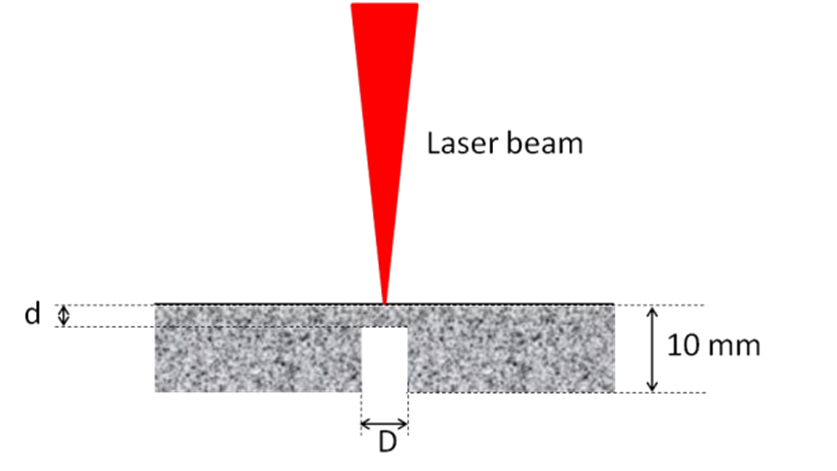
\includegraphics[width=0.3\linewidth]{./Figure/Figure2/a.png}}\hfill
	\subfigure[]{\label{subfig:2b}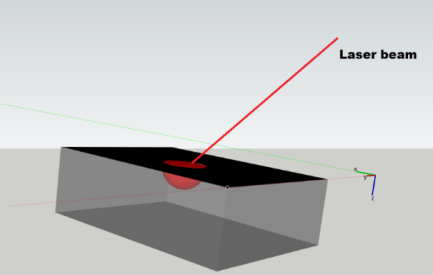
\includegraphics[width=0.3\linewidth]{./Figure/Figure2/b.png}} 
	\hspace*{\fill} \\ \hspace*{\fill}
	\subfigure[]{\label{subfig:2c}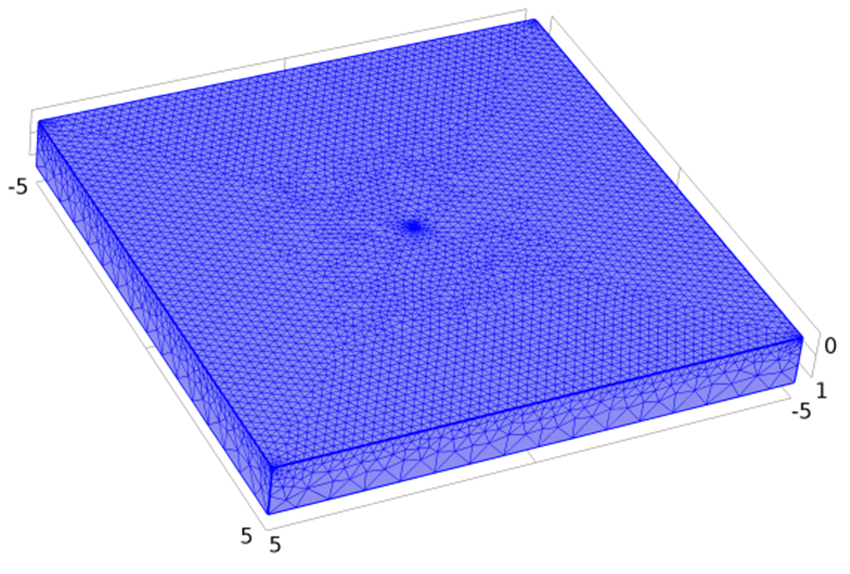
\includegraphics[width=0.3\linewidth]{./Figure/Figure2/c.png}}\hfill
	\subfigure[]{\label{subfig:2d}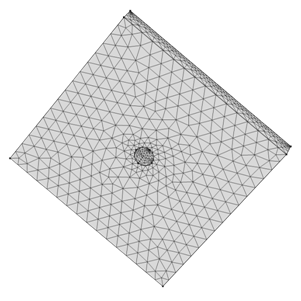
\includegraphics[width=0.3\linewidth]{./Figure/Figure2/d.png}}
	\hspace*{\fill}
    
	
		\caption{(a) Cross-sectional view of the geometry - (b) 3D Thermal response to a laser 
	excitation - (c) Geometry and meshing (front side), dimensions appears in cm  - (d) 
	Geometry and meshing (back side).}
  \label{fig:2}
\end{figure}


Furthermore, the black paint layer is considered as a dielectric material so that the energy provided by the interaction between the laser beam and material involves an absorption coefficient $\alpha$, near 1.
Transient conduction analysis of $heat$ $transfer$ $module$ has been selected to solve heat equation. The 2D geometry of the problem is represented in Fig.\,\ref{subfig:2a} where $d$ is the defect depth, $D$ is the defect diameter. Boundary condition imposed to all surfaces is in form of the following equation:

\begin{equation}
  \label{eq:33}
  n(k \nabla T) = \alpha q_0 + h(T_{ext} - T) \ ,
\end{equation}

\noindent where $n$ is the normal vector, $\alpha$ the absorption coefficient, $q_0$ is the inward heat flux on top surface and is equal to 0 on other surfaces, $h$ is a coefficient representing heat transfer losses due to convective heat flux with surrounding atmosphere. $h$ is equal to \SI{5}{\watt \per \square \metre \per \kelvin} on all surfaces, except on the surfaces of the defect where it is equal to 0 to simulate thermal insulation. $T_{ext}$ is the surrounding atmosphere temperature and it is assumed that the radiation heat transfer losses are neglected. 

For meshing, free tetrahedral meshes are selected with choice of a custom element size. The maximum element size is equal to \SI{0.032}{\milli \metre} with a maximum element growth rate equal to 1.35. The smallest element size is obtained near to the origin (0, 0, 0) centrally located on top of the surface (see Fig.\,\ref{subfig:2c}). A fine meshing is constructed with a number of elements ranging from $75,000$ to $225,000$ due to the presence of a \SI{0.1}{\milli \metre} layer on top of the simulated object surface. Furthermore, the system to solve consists of a number of degrees of freedom ranging from $111,000$ to $324,000$ and depends of the chosen geometry. Record time stepping is selected to \SI{0.1}{\second} in a range from \SI{0}{\second} to \SI{2}{\second}. Geometric Multigrid GMRES iterative linear solver is used. Backward Differentiation Formula (BDF) implicit method is used to help solver to converge.

	%

  \begin{figure}
  \centering
	

  \hspace*{\fill}
  \subfigure[]{\label{subfig:3a}\includegraphics[width=0.3\linewidth]{./Figure/Figure3/fig2d.png}} \hfill
  \subfigure[]{\label{subfig:3b}\includegraphics[width=0.3\linewidth]{./Figure/Figure3/fig2e.png}} 
  \subfigure[]{\label{subfig:3c}\includegraphics[width=0.3\linewidth]{./Figure/Figure3/fig2f.png}} 
	\hspace*{\fill} \\ \hspace*{\fill}
  \subfigure[]{\label{subfig:3d}\includegraphics[width=0.3\linewidth]{./Figure/Figure3/1.png}} \hfill
  \subfigure[]{\label{subfig:3e}\includegraphics[width=0.3\linewidth]{./Figure/Figure3/2.png}} 
  \subfigure[]{\label{subfig:3f}\includegraphics[width=0.3\linewidth]{./Figure/Figure3/3.png}} 
  \hspace*{\fill}
	
	  \caption{(a) and (d) Thermal response, observed on a non-defective area - (b) and (e) 
	Thermal response, observed on an area with defect of 1 mm below surface - (c) and (f) 
	Thermal response, 
	observed on an area with defect of 0.5 mm below surface.}
	
  \label{fig:3}
\end{figure}


  
  %\begin{figure}
  %\centering
  %\hspace*{\fill}
  %\subfigure[]{\label{subfig:3a}\includegraphics[width=0.3\linewidth]{fig2d.png}} \hfill
  %\subfigure[]{\label{subfig:3b}\includegraphics[width=0.3\linewidth]{fig2e.png}} 
  %\subfigure[]{\label{subfig:3c}\includegraphics[width=0.3\linewidth]{fig2f.png}} 
	%\hspace*{\fill} \\ \hspace*{\fill}
  %\subfigure[]{\label{subfig:3d}\includegraphics[width=0.3\linewidth]{1.png}} \hfill
  %\subfigure[]{\label{subfig:3e}\includegraphics[width=0.3\linewidth]{2.png}} 
  %\subfigure[]{\label{subfig:3f}\includegraphics[width=0.3\linewidth]{3.png}} 
  %\hspace*{\fill}
  %\caption{(a) and (d) Thermal response, observed on a non-defective area - (b) and (e) 
	%Thermal response, observed on an area with defect of 1 mm below surface - (c) and (f) 
	%Thermal response, 
	%observed on an area with defect of 0.5 mm below surface.}
  %\label{fig:3}
%\end{figure}


The interaction of the laser beam with the solid surface produces a thermal wave propagating through the solid media. In the case of a media without any defects and assuming a semi-infinite and isotropic solid, the thermal response is defined by the shape of a symmetric hemisphere\cite{Li2011} as shown in Fig.\,\ref{subfig:2b}. This response is modified due to the presence of a defect close to the excited area.

The simulation results are depicted in Fig.\,\ref{subfig:3a}-\ref{subfig:3b}-\ref{subfig:3c} by representing the temperature distribution in kelvin. It can be noted that the temperature intensity increases when the laser heats the defective area. Subsequently, the maximum temperature is reached for defects nearer to the surface. Fig.\,\ref{subfig:3d}-\ref{subfig:3e}-\ref{subfig:3f} represent the thermal response using another color-map. It can be observed that the amount of the thermal response increases due to the presence of inhomogeneities in the solid media.
	
\subsubsection{Defect detection algorithm}\label{subsec:312}
% \graphicspath{{./Figure/Figure4/}}
..
- defect.png                                                   [I]  2.91K !15/10/16 13:41

%
\begin{figure}
  \centering



  % Define the properties of the different blocks
  \tikzstyle{module}=[draw, draw=blue!80, text width=10em, 
  text centered, minimum height=5em, minimum width = 15em, drop shadow, rounded corners,
  fill=blue!30]

  \tikzstyle{vecArrow} = [thick, decoration={markings,mark=at position
    1 with {\arrow[semithick]{open triangle 60}}},
  double distance=1.4pt, shorten >= 5.5pt,
  preaction = {decorate},
  postaction = {draw,line width=1.4pt, white,shorten >= 4.5pt}]

  % Define distances for bordering
  \def\blockdist{1.5}
  \def\edgedist{2.5}

  \begin{tikzpicture}[node distance=3cm,thick,scale=0.4, every node/.style={scale=0.4},path image/.style={
      path picture={
        \node at (path picture bounding box.center) {
          \includegraphics[width=1cm]{#1}
        };}}]
    \tikzstyle{conefill} = [path image=,fill opacity=0.8]

    % First block with the pre-processing
    \node[module=above:pre] (pre) at (4.5,-2.6) {\Large Background\\ Subtraction};
    \node[module,below of=pre] (seg) {\Large Noise\\ Reduction};
    \node[module,below of=seg] (reg) {\Large Contrast\\ Enhancement};
    \draw[->] (pre)--(seg);
    \draw[->] (seg)--(reg);
    \begin{pgfonlayer}{background}
      \path (pre.west |- pre.north)+(-0.9,1.0+\blockdist) node (a) {};
      \path (reg.east |- reg.south)+(+0.9,-0.5) node (b) {};
      
      \path[fill=blue!10,rounded corners, draw=blue!20, dashed] (a) rectangle (b);
    \end{pgfonlayer}
    \path (pre.north) +(0,+\blockdist) node (bgreg) {\Large Pre-processing};

    % Second block with the segmentation
    \begin{scope}[node distance=3cm]
      \node[module] (det) [right=0cm and 2cm of seg] {\Large Region\\Growing};
    \end{scope}
    \begin{pgfonlayer}{background}
      \path (det.west |- det.north)+(-0.9,1.0+\blockdist) node (c) {};
      \path (det.east |- det.south)+(+0.9,-0.5) node (d) {};
      \path[fill=blue!10,rounded corners, draw=blue!20, dashed] (c) rectangle (d);
    \end{pgfonlayer}

    \path (det.north) +(0,+\blockdist) node (bgreg) {\Large Segmentation};

    % % Define the place where the arrow should start anf finish
    % \path (seg.east |- seg.north)+(+0.9,0) node (e) {};
    % \path (det.west |- seg.north)+(-0.8,0) node (f) {};

    % \draw[double distance =3pt,preaction={-triangle 90,thin,draw,shorten >=-1mm}] (e) -- (f) node[midway,above] {\Large Regularized data};

    % Third block with the merging
    \begin{scope}[node distance=3cm]
      \node[module] (mer) [right=0cm and 2cm of det] {\Large Merging};
    \end{scope}
    \node[module,below of=mer] (bin) {\Large Binarization};
    \begin{pgfonlayer}{background}
      \path (mer.west |- mer.north)+(-0.9,1.0+\blockdist) node (c) {};
      \path (bin.east |- bin.south)+(+0.9,-0.5) node (d) {};
      \path[fill=blue!10,rounded corners, draw=blue!20, dashed] (c) rectangle (d);
    \end{pgfonlayer}

    \path (mer.north) +(0,+\blockdist) node (bgreg) {\Large Detection};

    \draw[->] (mer)--(bin);

    \begin{scope}[yshift=-170,xshift=950]
      \transparent{1.0}\draw[path image=defect.png] (0,0) rectangle (1.0,1.0);
      \path (0,0)+(0.5,1.6) node {\Large Det. Img.};
    \end{scope}

    \begin{scope}[yshift=-132,xshift=594]
      \transparent{0.6}\draw[path image=rg.png] (0,0) rectangle (1.0,1.0);
    \end{scope}

    \begin{scope}[yshift=-136,xshift=600]
      \transparent{0.6}\draw[path image=rg.png] (0,0) rectangle (1.0,1.0);
    \end{scope}

    \begin{scope}[yshift=-140,xshift=606]
      \transparent{0.8}\draw[path image=rg.png] (0,0) rectangle (1.0,1.0);
      \path (0,0)+(0.0,1.8) node {\Large Seg. Img.};
    \end{scope}

    \begin{scope}[yshift=-132,xshift=270]
      \transparent{0.6}\draw[path image=th_im.png] (0,0) rectangle (1.0,1.0);
    \end{scope}

    \begin{scope}[yshift=-136,xshift=276]
      \transparent{0.6}\draw[path image=th_im.png] (0,0) rectangle (1.0,1.0);
    \end{scope}

    \begin{scope}[yshift=-140,xshift=282]
      \transparent{0.8}\draw[path image=th_im.png] (0,0) rectangle (1.0,1.0);
      \path (0,0)+(0.0,1.8) node {\Large Enh. Img.};
    \end{scope}

    \begin{scope}[yshift=-166,xshift=-82]
      \transparent{0.6}\draw[path image=th_im_2.png] (0,0) rectangle (1.0,1.0);
    \end{scope}

    \begin{scope}[yshift=-172,xshift=-76]
      \transparent{0.6}\draw[path image=th_im_2.png] (0,0) rectangle (1.0,1.0);
    \end{scope}

    \begin{scope}[yshift=-176,xshift=-70]
      \transparent{0.8}\draw[path image=th_im_2.png] (0,0) rectangle (1.0,1.0);
      \path (0,0)+(0.0,1.8) node {\Large Thermal Image};
    \end{scope}

    \path (seg.west |- seg.north)+(-2.5,-1) node (i) {};
    \path (seg.west |- seg.north)+(-0.9,-1) node (j) {};
    \draw[double distance =3pt,preaction={-triangle 90,thin,draw,shorten >=-1mm}] (i) -- (j);
    
    \path (seg.east |- seg.north)+(0.9,-1) node (ii) {};
    \path (det.west |- det.north)+(-0.9,-1) node (jj) {};
    \draw[double distance =3pt,preaction={-triangle 90,thin,draw,shorten >=-1mm}] (ii) -- (jj);

    \path (det.east |- det.north)+(0.9,-1) node (ii) {};
    \path (mer.west |- mer.north)+(-0.9,-1) node (jj) {};
    \draw[double distance =3pt,preaction={-triangle 90,thin,draw,shorten >=-1mm}] (ii) -- (jj);

    \path (mer.east |- mer.north)+(0.9,-1) node (ii) {};
    \path (mer.east |- mer.north)+(2.5,-1) node (jj) {};
    \draw[double distance =3pt,preaction={-triangle 90,thin,draw,shorten >=-1mm}] (ii) -- (jj);   
    
  \end{tikzpicture}



  \caption{Image processing work-flow to detect non-through defects.}
  \label{fig:wkdetection}
\end{figure}


The object surface is punctually scanned using a laser beam and at each of these scans, a thermal image is acquired (see Fig.\,\ref{subfig:44c}).
Defect localization is characterized by a change of the heat distribution and therefore can be detected with an appropriate image processing algorithm in the thermal images.
Our developed framework is depicted in Fig.\,\ref{fig:wkdetection} and can be subdivided into three stages: (i) pre-processing, (ii) segmentation, and (iii) detection.

\paragraph{Pre-processing} Each acquired thermal image is enhanced by successively subtracting the background, reducing the noise, and stretching the contrast. The background to be subtracted consists in the acquisition of a thermal image before laser stimulation. Additionally, a median filtering is applied to the image to reduce the noise and the denoised image is enhanced through contrast stretching.
\paragraph{Segmentation} Then, the enhanced image is segmented using the region growing segmentation algorithm~\cite{Adams1994}. 
The initial seed point is automatically placed on the center of the thermal response corresponding to the maximum temperature in the image.
Then, the region grows if the difference of temperature values of the neighboring pixels and the region's mean is less than a given region membership criterion.
The pixel with the smallest difference is assigned to the segmented region.
\paragraph{Detection} The detection is subdivided into two stages: (i) merging and (ii) binarization.
All segmented images are combined together by creating a matrix $s$ such that the number of white pixels of a given segmented image is assigned to the location $(i,j)$, which corresponds to the location of the laser stimulation.
Subsequently, to limit the influence of the emissivity change and detect robustly the defective area, the median $\tilde{s}$ is computed for each \ac{roi} with a size $(40\times40)$ and compared to each value $s(i,j)$ inside this \ac{roi} in order to binarize $s$:

\begin{equation}
  \label{eq:3}
s_m(i,j) = \begin{cases}
1 & \quad \text{if } s(i,j) \geq K \times \tilde{s}\\
0 & \quad \text{if } s(i,j) < K \times \tilde{s}
\end{cases}
\end{equation}

\noindent where $K > 1$ and $s_m(i,j)$ is the resulting binary mask of the defects detection.
If $K \gg 1$, the defect detection is more robust to noise. However, only shallowest defect are detected; if $K \to 1$, the defect detection is subject to noise. However, deeper defect are detected.

\subsection{Fiber orientation assessment}\label{subsec:32}

	%
\graphicspath{{./Figure/Figure5/}}
\begin{figure}
  \centering
	
  % Define the properties of the different blocks
  \tikzstyle{module}=[draw, draw=blue!80, text width=10em, 
  text centered, minimum height=5em, minimum width = 15em, drop shadow, rounded corners,
  fill=blue!30]

  \tikzstyle{vecArrow} = [thick, decoration={markings,mark=at position
    1 with {\arrow[semithick]{open triangle 60}}},
  double distance=1.4pt, shorten >= 5.5pt,
  preaction = {decorate},
  postaction = {draw,line width=1.4pt, white,shorten >= 4.5pt}]

  % Define distances for bordering
  \def\blockdist{1.5}
  \def\edgedist{2.5}

  \begin{tikzpicture}[node distance=3cm,thick,scale=0.4, every node/.style={scale=0.4},path image/.style={
      path picture={
        \node at (path picture bounding box.center) {
          \includegraphics[width=1cm]{#1}
        };}}]
    \tikzstyle{conefill} = [path image=,fill opacity=0.8]

    % First block with the pre-processing
    %\node[module=above:pre] (pre) at (4.5,-2.6) {\Large Background\\ Subtraction};
    \node[module=above:seg] (seg) at (4.5,-2.6) {\Large Background\\ Subtraction};
    %\node[module,below of=seg] (reg) {\Large Contrast\\ Enhancement};
    %\draw[->] (pre)--(seg);
    %\draw[->] (seg)--(reg);
    \begin{pgfonlayer}{background}
      \path (seg.west |- seg.north)+(-0.9,1.0+\blockdist) node (a) {};
      \path (seg.east |- seg.south)+(+0.9,-0.5) node (b) {};
      
      \path[fill=blue!10,rounded corners, draw=blue!20, dashed] (a) rectangle (b);
    \end{pgfonlayer}
    \path (pre.north) +(0,+\blockdist) node (bgreg) {\Large Pre-processing};

    % Second block with the segmentation
    \begin{scope}[node distance=3cm]
      \node[module] (det) [right=0cm and 2cm of seg] {\Large Region\\Growing};
    \end{scope}
    \node[module,below of=det] (can) {\Large Canny\\ Edge Detector};
    \begin{pgfonlayer}{background}
      \path (det.west |- det.north)+(-0.9,1.0+\blockdist) node (c) {};
      \path (can.east |- can.south)+(+0.9,-0.5) node (d) {};
      \path[fill=blue!10,rounded corners, draw=blue!20, dashed] (c) rectangle (d);
    \end{pgfonlayer}

    
    \draw[->] (det)--(can);

    \path (det.north) +(0,+\blockdist) node (bgreg) {\Large Segmentation};

    % % Define the place where the arrow should start anf finish
    % \path (seg.east |- seg.north)+(+0.9,0) node (e) {};
    % \path (det.west |- seg.north)+(-0.8,0) node (f) {};

    % \draw[double distance =3pt,preaction={-triangle 90,thin,draw,shorten >=-1mm}] (e) -- (f) node[midway,above] {\Large Regularized data};

    % Third block with the merging
    \begin{scope}[node distance=3cm]
      \node[module] (mer) [right=0cm and 2cm of det] {\Large Algebraic\\ Fitting};
    \end{scope}
    \begin{pgfonlayer}{background}
      \path (mer.west |- mer.north)+(-0.9,1.0+\blockdist) node (c) {};
      \path (mer.east |- mer.south)+(+0.9,-0.5) node (d) {};
      \path[fill=blue!10,rounded corners, draw=blue!20, dashed] (c) rectangle (d);
    \end{pgfonlayer}

    \path (mer.north) +(0,+\blockdist) node (bgreg) {\Large Fitting};

    \begin{scope}[yshift=-85,xshift=950]
      \transparent{1.0}\draw[path image=fig9d.png] (0,0) rectangle (1.0,1.0);
      \path (0,0)+(0.5,1.6) node {\Large Det. Img.};
    \end{scope}

    \begin{scope}[yshift=-60,xshift=606]
      \transparent{1.0}\draw[path image=fig9c.png] (0,0) rectangle (1.0,1.0);
      \path (0,0)+(0.0,1.8) node {\Large Seg. Img.};
    \end{scope}

    \begin{scope}[yshift=-60,xshift=282]
      \transparent{1.0}\draw[path image=th_im.png] (0,0) rectangle (1.0,1.0);
      \path (0,0)+(0.0,1.8) node {\Large Enh. Img.};
    \end{scope}

    \begin{scope}[yshift=-85),xshift=-70]
      \transparent{1.0}\draw[path image=th_im_2.png] (0,0) rectangle (1.0,1.0);
      \path (0,0)+(0.0,1.8) node {\Large Thermal Image};
    \end{scope}

    \path (seg.west |- seg.north)+(-2.5,-1) node (i) {};
    \path (seg.west |- seg.north)+(-0.9,-1) node (j) {};
    \draw[double distance =3pt,preaction={-triangle 90,thin,draw,shorten >=-1mm}] (i) -- (j);
    
    \path (seg.east |- seg.north)+(0.9,-1) node (ii) {};
    \path (det.west |- det.north)+(-0.9,-1) node (jj) {};
    \draw[double distance =3pt,preaction={-triangle 90,thin,draw,shorten >=-1mm}] (ii) -- (jj);

    \path (det.east |- det.north)+(0.9,-1) node (ii) {};
    \path (mer.west |- mer.north)+(-0.9,-1) node (jj) {};
    \draw[double distance =3pt,preaction={-triangle 90,thin,draw,shorten >=-1mm}] (ii) -- (jj);

    \path (mer.east |- mer.north)+(0.9,-1) node (ii) {};
    \path (mer.east |- mer.north)+(2.5,-1) node (jj) {};
    \draw[double distance =3pt,preaction={-triangle 90,thin,draw,shorten >=-1mm}] (ii) -- (jj);   
    
  \end{tikzpicture}

  
	\caption{Image processing work-flow to infer the fiber orientation.}
  \label{fig:wkfiber}
\end{figure}

%%% Local Variables:
%%% mode: latex
%%% TeX-master: "../../../master"
%%% End:


The fiber orientation is estimated based on the pulsed thermal ellipsometry approach~\cite{Cielo1987}.
Indeed, the thermal response of a polymer matrix composite material stimulated by a laser beam is elliptic due to the propagation of the heat through the fiber.
The framework developed to infer the fiber orientation is depicted in Fig.\,\ref{fig:wkfiber}.
Thermal images are acquired with an IR camera and are pre-processed with the following steps: (i) background subtraction, (ii) a segmentation using region growing, and (iii) an edge detection using Canny edge detector~\cite{Canny1986}. 
Three methods are commonly used to fit an ellipse: (i) algebraic fitting~\cite{Fitzgibbon1999}, (ii) orthogonal least squares fitting~\cite{Ahn2001}, and (iii) Maximum Likelihood algorithms~\cite{Chojnacki2000}. 
The two latter methods are suitable for 3D data, whereas the first method can only be applied to 2D problems.
Algebraic fitting, however, offers a low computational complexity and is suitable in our case.
In this method, the ellipse is formulated by the general conic polynomial:

\begin{equation}
  \label{eq:4}
  F(a, X) = aX = 0 \,
\end{equation}

\noindent with 

\begin{eqnarray}
  a & = & \begin{bmatrix} A & B & C & D & E & F \\ \end{bmatrix}^\intercal \nonumber\\
  X & = & \begin{bmatrix} x^2 & xy & y^2 & x & y & 1 \\ \end{bmatrix}^\intercal \nonumber
\end{eqnarray}

The fitting is performed by a least square minimization of the Euclidean distances such that:

\begin{equation}
  \argmin{a} \sum_{i=1}^{n} \left( A x_i^2 + B x_i y_i + C y_i^2 + D x_i + E Y_i + F \right)^2 \ .
\end{equation}

The following constraint yields to one solution which corresponds to an ellipse:


% \include*{content/exp/exp}
\graphicspath{ {./content/exp/figure/} }

\section{Experiments and results}\label{sec:4}

\subsection{Experimental setup}


	%\graphicspath{ {./Figure/Figure6/} }
\begin{figure}
  \centering
  \hspace*{\fill}
  %\subfigure[]{\label{subfig:4a}\includegraphics[width=0.3\linewidth]{fig4a.png}} \hfill
  %\subfigure[]{\label{subfig:4b}\includegraphics[width=0.3\linewidth]{fig4b.png}} 
  %\hspace*{\fill} \\ \hspace*{\fill}
  %\subfigure[]{\label{subfig:4c}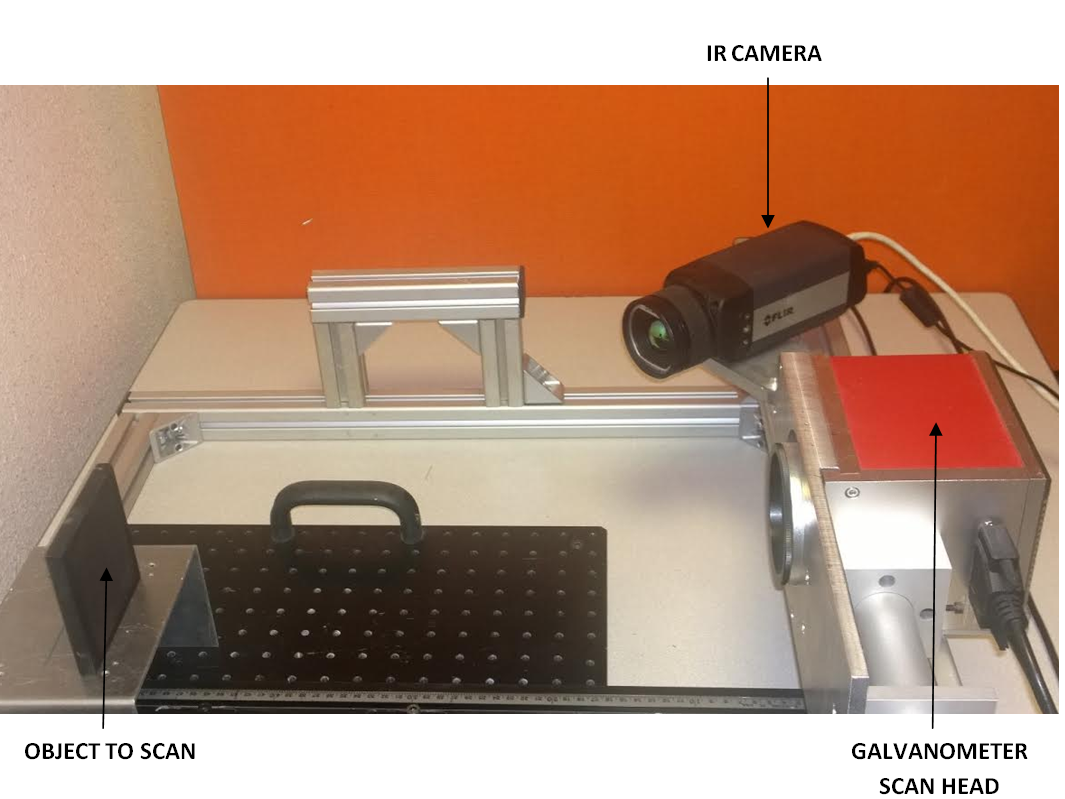
\includegraphics[width=0.3\linewidth]{fig4c.png}}
	{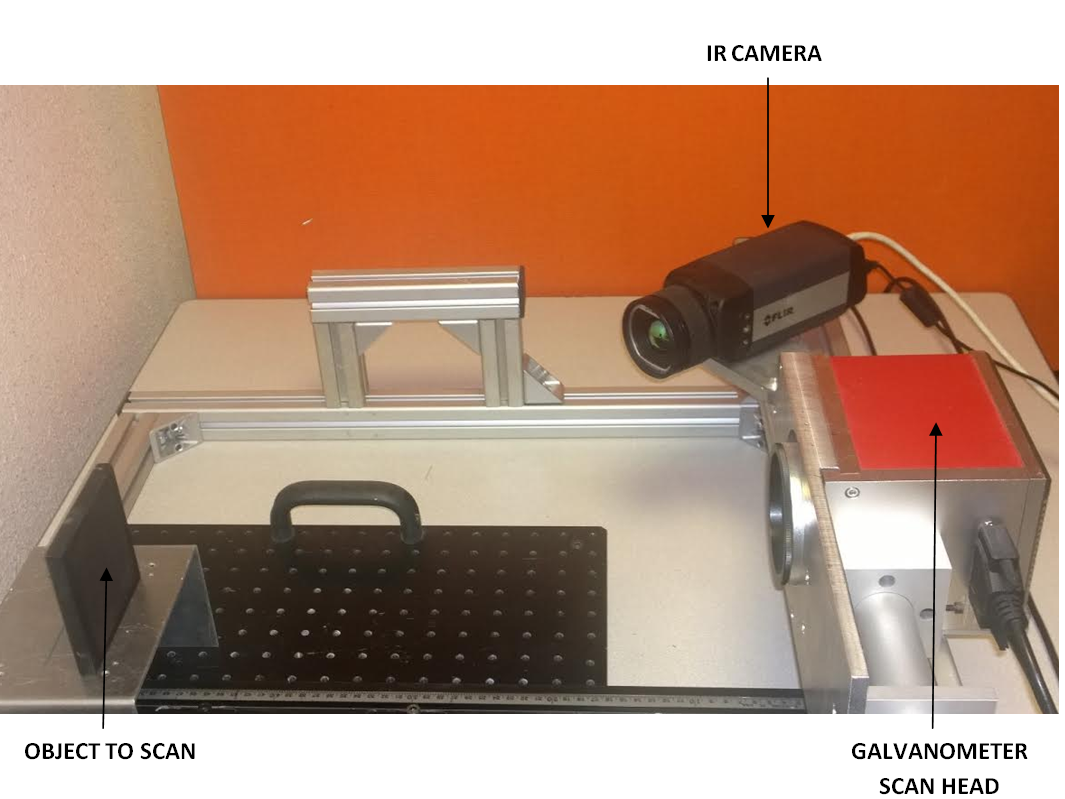
\includegraphics[width=0.7\linewidth]{fig4c.png}}
  \hspace*{\fill}
	
	\caption{Scanner prototype.}
  \label{fig:4}
\end{figure}
  

%\begin{figure}
  %\centering
  %\hspace*{\fill}
  %%\subfigure[]{\label{subfig:4a}\includegraphics[width=0.3\linewidth]{fig4a.png}} \hfill
  %%\subfigure[]{\label{subfig:4b}\includegraphics[width=0.3\linewidth]{fig4b.png}} 
  %%\hspace*{\fill} \\ \hspace*{\fill}
  %%\subfigure[]{\label{subfig:4c}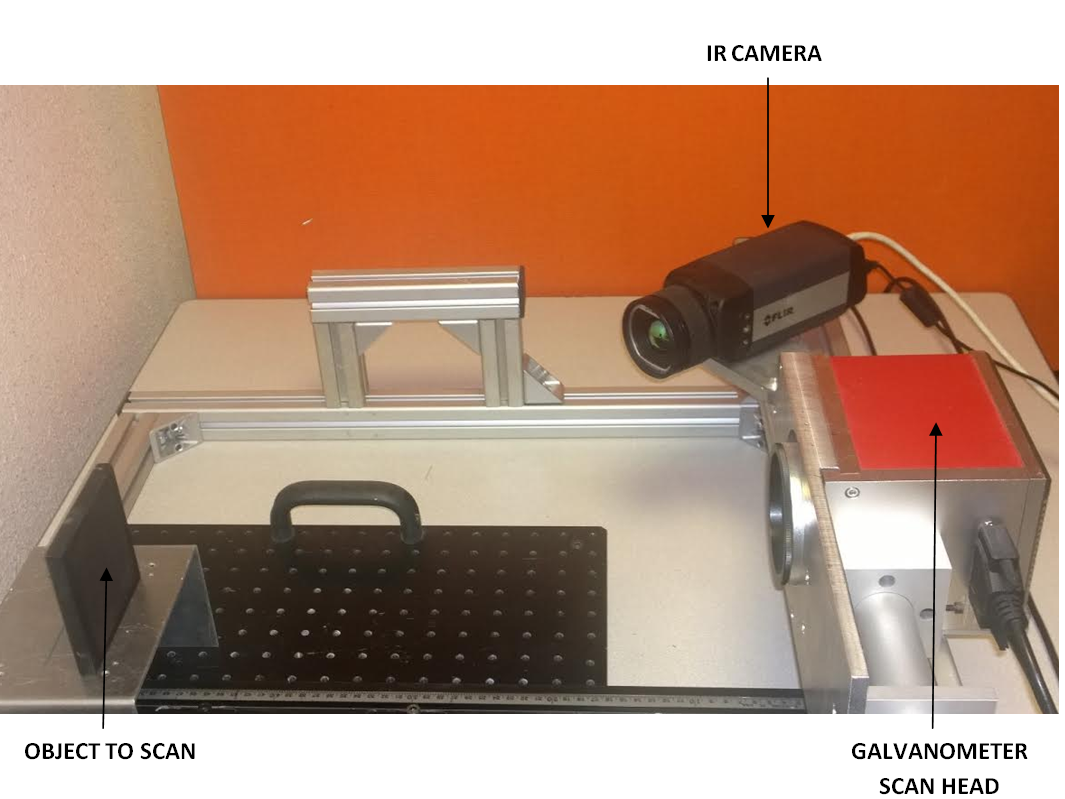
\includegraphics[width=0.3\linewidth]{fig4c.png}}
	%{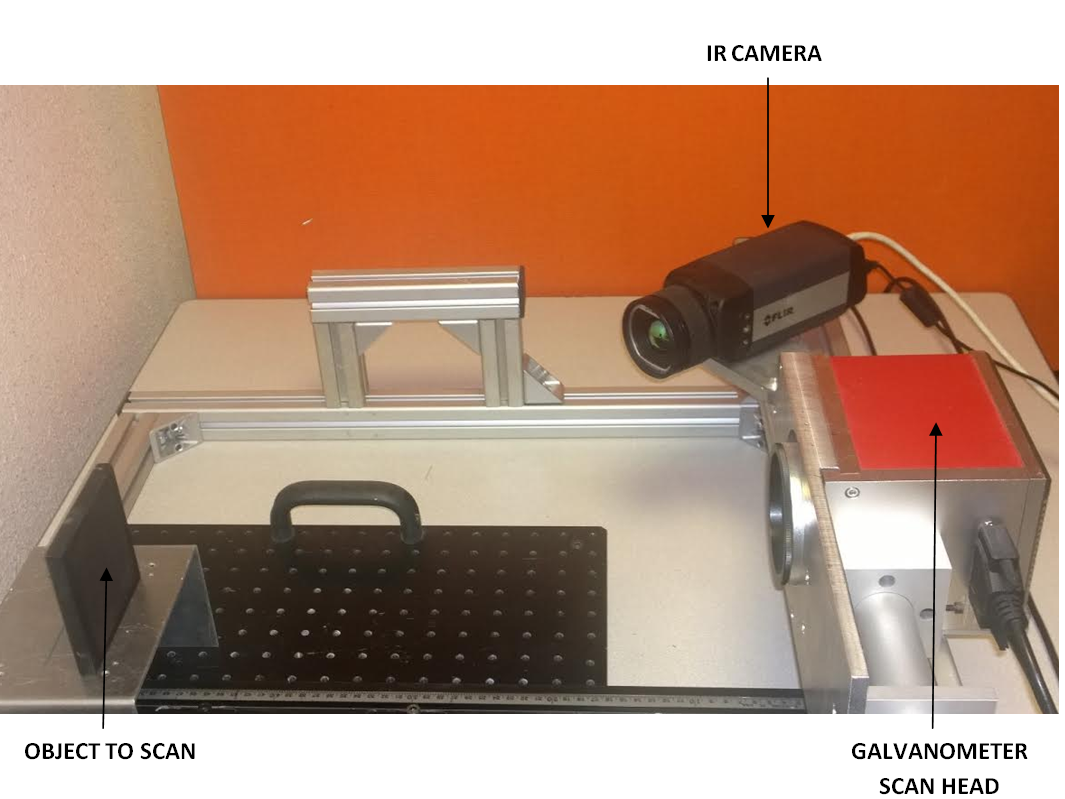
\includegraphics[width=0.7\linewidth]{fig4c.png}}
  %\hspace*{\fill}
  %\caption{%(a)-(b) Device for positioning the composite material - 
	%Scanner prototype.}
  %\label{fig:4}
%\end{figure}

Figure~\ref{fig:4} illustrates the complete scanning system setup. The system is composed by a FLIR~645 IR camera which captures the thermal radiation and an Nd~:YAG Laser system to stimulate the object surface. 
The FLIR~645 infrared camera provides a sensitivity range from \numrange{7.5}{14} \si{\micro \metre}.
The Nd~:YAG Laser system produces a step signal of \SI{1.5}{\second} period and the power of the laser beam is set up at \SI{1.5}{\watt}. 
A galvanometric mirror is used to control the position of the beam, which facilitates the object scanning with a \SI{1}{\milli \metre} resolution. 
During the experiment regarding the fiber orientation assessment, the motorized rotary stage ZABER T-RS60A is used.

\subsection{Experimental temperature profile}\label{subsec:42}

In order to validate the simulation results presented in Sect.\,\ref{subsec:311}, a set of thermal images are acquired. 
In these images, a defective area with a defect of \SI{0.5}{\milli \metre} below the surface and non-defective areas are excited with the laser beam (see Fig.\,\ref{fig:44}).
As previously predicted in the simulation section, the thermal response of a defective-area is different from the non-defective area, allowing non-through defects detection.

\subsection{Non-through defect detection}

%Figure~\ref{fig:5} reports two pairs of thermal images and their associated segmentation. The area of the segmented region in the image is more important when the laser impinges on a defective region of the object. By applying the segmentation method described in Sect.\,\ref{subsec:31}, we can detect the defective areas on the object's surface. 

Two type of material are used for the non-through defect detection: (i) steal plate and (ii) aluminum plate.
Both type of plates have non-through artificial defects, i.e. circle, square, triangle, and cross.
Defects are located between \SI{0.5}{\milli \metre} and \SI{2}{\milli \metre} below the observed surface for the aluminum plate and between \SI{1}{\milli \metre} and \SI{3}{\milli \metre} in the case of the steel plate.
The images are processed with the image processing algorithm presented in Sect.\,\ref{subsec:312}.
A 4-neighbors is considered during the region growing algorithm and a membership criterion of $0.2$, while the matrix $s_m$ is generated with $K=1.4$.
The results are depicted in Fig.\,\ref{fig:6} by superimposing with a color map on the raw image (i.e., red pixels are the non-through defects).

	%\graphicspath{ {./Figure/Figure7/} }
\begin{figure}
  \centering
	
  \hspace*{\fill}
  \subfigure[]{\label{subfig:44a}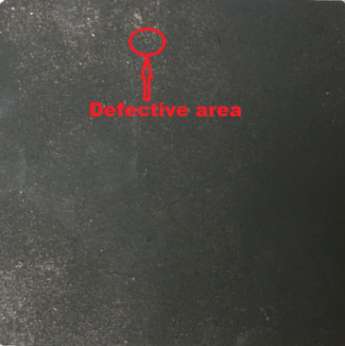
\includegraphics[width=0.3\linewidth]{fig3a.png}} \hfill
  \subfigure[]{\label{subfig:44b}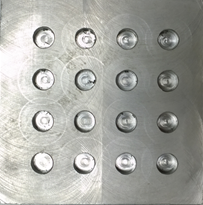
\includegraphics[width=0.3\linewidth]{fig3b.png}} 
  \hspace*{\fill} \\ \hspace*{\fill}
  \subfigure[]{\label{subfig:44c}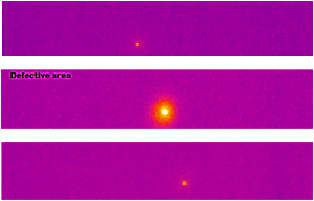
\includegraphics[width=0.3\linewidth]{fig3c.png}}
  %\subfigure[]{\label{subfig:3d}\includegraphics[width=0.3\linewidth]{fig3d.png}}
  \hspace*{\fill}
	
	  \caption{(a) Front side of the inspected material - (b) Back side of the inspected
		material - (c) Form of the thermal response of the material in the area with and without
		defect.}
		\label{fig:44}
		\end{figure}
  
	


%\begin{figure}
  %\centering
  %\hspace*{\fill}
  %\subfigure[]{\label{subfig:44a}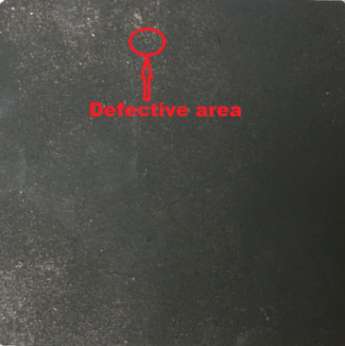
\includegraphics[width=0.3\linewidth]{fig3a.png}} \hfill
  %\subfigure[]{\label{subfig:44b}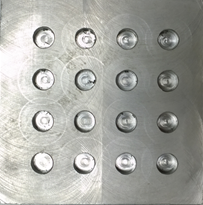
\includegraphics[width=0.3\linewidth]{fig3b.png}} 
  %\hspace*{\fill} \\ \hspace*{\fill}
  %\subfigure[]{\label{subfig:44c}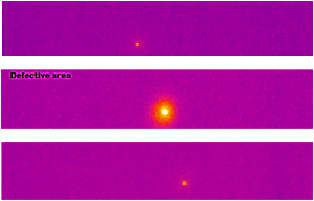
\includegraphics[width=0.3\linewidth]{fig3c.png}}
  %%\subfigure[]{\label{subfig:3d}\includegraphics[width=0.3\linewidth]{fig3d.png}}
  %\hspace*{\fill}
  %\caption{(a) Front side of the inspected material - (b) Back side of the inspected material 
	%- (c) Form of the thermal response of the material in the area with and without defect.}
  %\label{fig:44}
%\end{figure}

Figure~\ref{subfig:6a} shows a steel plate with circular non-through defects, in which defects have a diameter of 9, 7, 5, and \SI{3}{\milli \metre}, from left to right. 
Each defect is positioned at a different depth 1, 2, 2.5, and \SI{3}{\milli \metre}, from bottom to top. 
Only defects with depth less than or equal to \SI{2.5}{\milli \metre} are detected. 
However, the defects with a diameter less than \SI{5}{\milli \metre} are not detected as shown in Fig.\,\ref{subfig:6b}.
Besides, for the aluminum plate all defects are detected and the shape of the defect can be distinguished (see Fig.\,\ref{subfig:6d}). 

	%\graphicspath{ {./Figure/Figure8/}}
\begin{figure}
  \centering
	

  \hspace*{\fill}
  %\subfigure[]{\label{subfig:6a}\includegraphics[width=0.3\linewidth]{fig6a.png}} \hfill
  %\subfigure[]{\label{subfig:6b}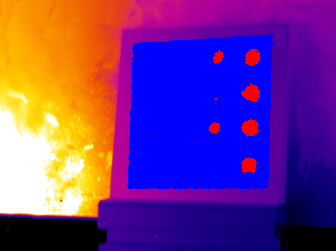
\includegraphics[width=0.3\linewidth]{fig6b.png}} 
  \subfigure[]{\label{subfig:6a}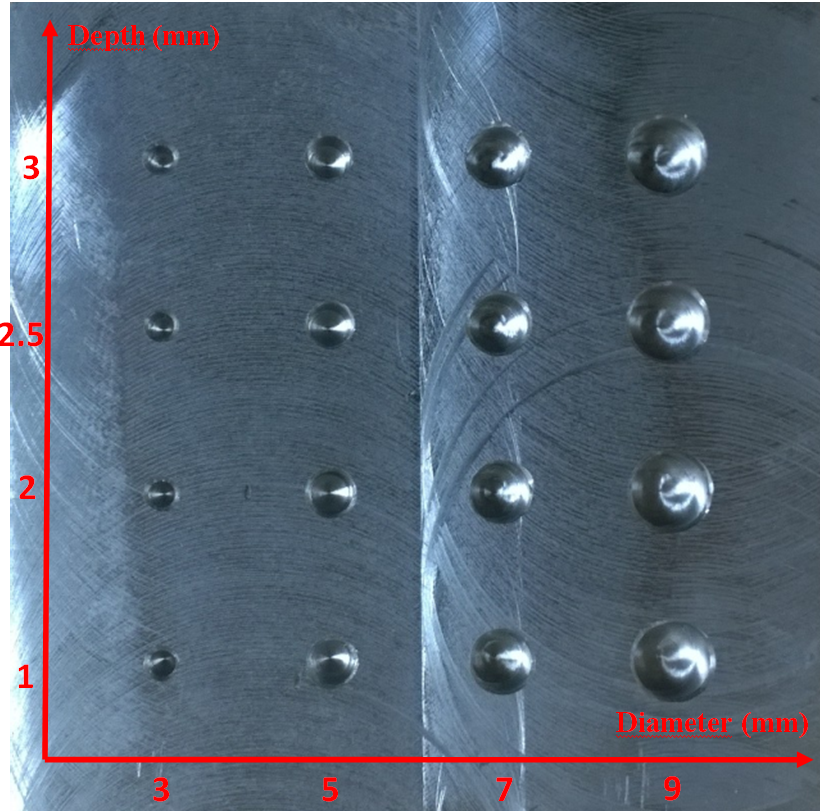
\includegraphics[width=0.3\linewidth]{fig7b.png}} \hfill
	\subfigure[]{\label{subfig:6b}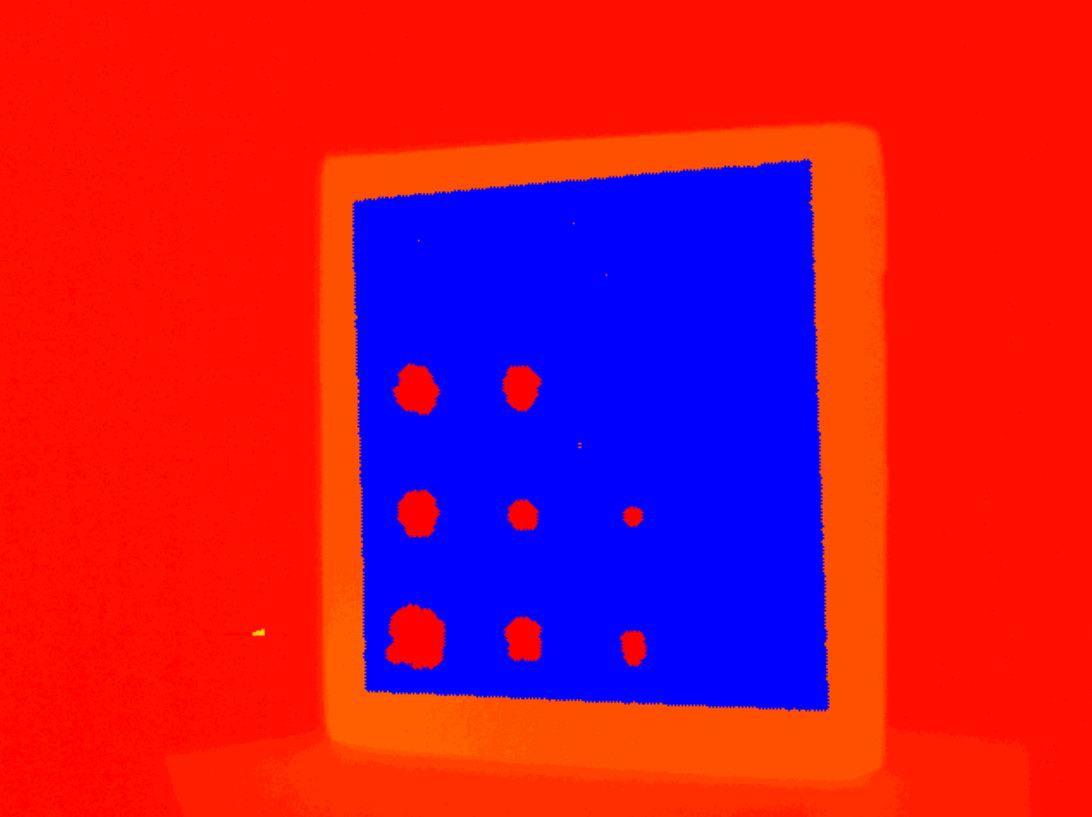
\includegraphics[width=0.3\linewidth]{fig7c.png}}
  \hspace*{\fill} \\ \hspace*{\fill}
  \subfigure[]{\label{subfig:6c}\includegraphics[width=0.3\linewidth]{fig6c.png}} \hfill
  \subfigure[]{\label{subfig:6d}\includegraphics[width=0.3\linewidth]{fig6d.png}}
  \hspace*{\fill}
	
	  \caption{(a) and (c) Steel and aluminum objects - (b) and (d) Corresponding detection map.}
		\label{fig:6}
		\end{figure}
  
 
%\begin{figure}
  %\centering
  %\hspace*{\fill}
  %%\subfigure[]{\label{subfig:6a}\includegraphics[width=0.3\linewidth]{fig6a.png}} \hfill
  %%\subfigure[]{\label{subfig:6b}\includegraphics[width=0.3\linewidth]{fig6b.png}} 
  %\subfigure[]{\label{subfig:6a}\includegraphics[width=0.3\linewidth]{fig7b.png}} \hfill
	%\subfigure[]{\label{subfig:6b}\includegraphics[width=0.3\linewidth]{fig7c.png}}
  %\hspace*{\fill} \\ \hspace*{\fill}
  %\subfigure[]{\label{subfig:6c}\includegraphics[width=0.3\linewidth]{fig6c.png}} \hfill
  %\subfigure[]{\label{subfig:6d}\includegraphics[width=0.3\linewidth]{fig6d.png}}
  %\hspace*{\fill}
  %\caption{(a) and (c) Steel and aluminum objects - (b) and (d) Corresponding detection map.}
  %\label{fig:6}
%\end{figure}

To study the repeatability of the technique, our framework is evaluated on steel plate with 16 identical circular defects located at \SI{1}{\milli \metre} depth and a \SI{10}{\milli \metre} diameter. 
The result of this experiment is depicted in Fig.\,\ref{subfig:7b}, in which all defects are successfully detected.


	%\graphicspath{ {./Figure/Figure9/}}
\begin{figure}
  \centering
	

  \hspace*{\fill}
  \subfigure[]{\label{subfig:7a}\includegraphics[width=0.3\linewidth]{fig7a.png}} \hfill
	\subfigure[]{\label{subfig:7b}\includegraphics[width=0.3\linewidth]{fig7d.png}} 
  \hspace*{\fill}


	
		\caption{(a) Steel objects - (b) Corresponding detection map.}
  \label{fig:7}
\end{figure}
  

\subsection{Fusion of defect localization and 3D data}

To assess the quality of the fusion between the defect localization and the 3D data, a steel object is scanned (see Fig.\,\ref{subfig:8a}) to acquire a set of thermal images.
The steel object contains non-through circular defects in the planar part with a depth of \SI{1}{\milli \metre}.
The scanned area corresponds to the highlighted red delimitation depicted in Fig.\,\ref{subfig:8a}.
A similar method as proposed by Bajard~\emph{et al.}~\cite{Bajard2012} is used to obtain the 3D information and the defects are detected as in Sect.\ref{subsec:311}.
The coordinate system is the same for the 3D and defects information due to the fact that these data are acquired with the same system.
Therefore, the fusion between these data is straightforward, which overcome the matching problem faced by other methods as stated in the introduction section.

	%\graphicspath{ {./Figure/Figure10/}}
\begin{figure}
  \centering
	
  \hspace*{\fill}
  \subfigure[]{\label{subfig:8a}\includegraphics[width=0.3\linewidth]{fig8a.png}}\hfill
  \subfigure[]{\label{subfig:8b}\includegraphics[width=0.3\linewidth]{fig8b.png}} 
	\hspace*{\fill} \\ \hspace*{\fill}
  \subfigure[]{\label{subfig:8c}\includegraphics[width=0.3\linewidth]{fig8c.png}} \hfill
  \subfigure[]{\label{subfig:8d}\includegraphics[width=0.3\linewidth]{fig8d.png}}
  \hspace*{\fill}
	
	\caption{(a) The specimen - (b) 3D mesh - (c) Corresponding detection map - (d) 3D mapping.}
  \label{fig:8}
\end{figure}
 

\subsection{Fiber orientations assessment}

In this section, we evaluate our framework at detecting the fiber orientation of carbon fiber composite material (see Fig.\,\ref{subfig:9a}).
The fiber orientation is estimated using the methodology presented in Sect.\,\ref{subsec:32}.
The initial experimental setup is as follows: 
firstly, the material is heated with the laser beam, the thermal radiation is recorded, and the orientation of the fiber is inferred. 
Secondly, the experiment is repeated by rotating the carbon plate at a \SI{90}{\degree} position.
The results of the ellipse fitting are depicted in Fig.\,\ref{subfig:9b}-\ref{subfig:9c}-\ref{subfig:9d}.
The algebraic fitting qualitatively shows an accurate fitting as shown in Fig.\,\ref{subfig:9d}, in which the blue dots represents the raw data, the green curve is the fitted ellipse, and the red line represents the ellipse major axis orientation.
As expected, the ellipse orientation follows the material rotation as depicted Fig.\,\ref{fig:10}.


	%\graphicspath{ {./Figure/Figure11/}}
\begin{figure}
  \centering
	

  \hspace*{\fill}
  \subfigure[]{\label{subfig:9a}\includegraphics[width=0.3\linewidth]{fig9a.png}}
  \hspace*{\fill} \\ \hspace*{\fill}
  \subfigure[]{\label{subfig:9b}\includegraphics[width=0.3\linewidth]{fig9b.png}} \hfill
  \subfigure[]{\label{subfig:9c}\includegraphics[width=0.3\linewidth]{fig9c.png}} \hfill
  \subfigure[]{\label{subfig:9d}\includegraphics[width=0.3\linewidth]{fig9d.png}}
  \hspace*{\fill}
	  
		\caption{(a) The specimen - (b) Segmented thermal response - (c) Edge of the thermal
		response - (d) Ellipse fitting.}
		\label{fig:9}
		\end{figure}
  


	
	%\graphicspath{ {./Figure/Figure12/}}
\begin{figure}
  \centering

  \hspace*{\fill}
  \subfigure[]{\label{subfig:10a}\includegraphics[width=0.3\linewidth]{fig10aa.png}} \hfill
  \subfigure[]{\label{subfig:10b}\includegraphics[width=0.3\linewidth]{fig10bb.png}} 
  \hspace*{\fill} \\ \hspace*{\fill}
  \subfigure[]{\label{subfig:10c}\includegraphics[width=0.3\linewidth]{fig10cc.png}} \hfill
  \subfigure[]{\label{subfig:10d}\includegraphics[width=0.3\linewidth]{fig10dd.png}}
  \hspace*{\fill}
	
	\caption{Example of fiber orientation detection: (a)-(b) horizontally oriented - (c)-(d)
		vertically oriented.}
		\label{fig:10}
		\end{figure}
  




The previous experiment are repeated acquiring 4 measurements for different orientations ranging from \SI{-10}{\degree} to \SI{-60}{\degree} with a step of \SI{10}{\degree}.
The absolute orientations are estimated and the mean and standard deviation are computed as presented in Table~\ref{tab:1}.
The average relative orientation is equal to \SI{10.8}{\degree} with a standard deviation of \SI{1.7}{\degree} and can be compared to the step which is set to \SI{10}{\degree}.


% \include*{content/conc/conc}
\newpage

\section{Conclusion and future works}\label{sec:5}

In this paper, a system based on the \ac{sfh} approach is proposed for detecting non-through defects and fiber orientation. 
In the one hand, experiments conducted on steel and aluminum plates showed that non-through defects until \SI{2.5}{\milli \metre} are detected. 
On the other hand, a test was carried out in order to investigate the influence of the depth and the size of the defects on the defect detection.
In addition, accurate fiber orientation assessment is achieved with an experimental standard deviation of \SI{1.7}{\degree}. 
The use of the \ac{sfh} for \ac{ndt} application and the 3D digitization offers the prospect to imagine an industrial system that can give a complete solution for quality control process. 
As future works, tests will be done on different specimen to explore the influence of material properties, defect size and depth on the detection method. 
Detecting defect on complex objects is a though challenge in active thermography. 
Our technique has proven to be effective for non-through defect detection on planar object. 
The next step is to investigate the possibility of detecting defects on complex geometry objects.   
Moreover, kinetic analysis of the thermal radiation could allow to estimate the depth of the defect.

% \include*{content/other/other}

\acknowledgments     %>>>> equivalent to \section*{ACKNOWLEDGMENTS}

This work is supported by the Regional Council of Burgundy. We are extremely grateful to members of laboratory LE2I for day to day help and collaboration.


\newpage
\bibliography{./Bibliography}   %>>>> bibliography data in report.bib
\bibliographystyle{spiejour}   %>>>> makes bibtex use spiebib.bst


\newpage
%\begin{description}

\vspace{2ex}\noindent\textbf{M. Belkacemi} received M.Sc. in Signal and Image processing delivered by the Pierre et Marie CURIE University (UPMC). 
He is currently carrying out a Ph.D. at the University of Burgundy. His research interests include active thermography for Non-Destructive Testing (NDT) and non conventional imaging systems for 3D digitization.

\vspace{2ex}\noindent\textbf{C. Stolz} received his M.Sc. degree in automatics and industrial computing system in 1995 from the Université de Haute Alsace, Mulhouse, France. He obtained his PhD in optical signal processing from the same university in 2000. In 2001, he was appointed to his position of assistant professor in the Computing, Electronic, Imaging Laboratory (LE2I) of the Universite de Bourgogne. His research interests mainly concern optical and digital image processing, more particularly polarimetric methods applied to shape measurement.

\vspace{2ex}\noindent\textbf{A. Mathieu} obtained a PhD from University of Burgundy, in 2005. Since 2008, he is lecturer at University of Burgundy. He is a member from laboratory “Interdisciplinaire Carnot de Bourgogne” (ICB UMR 6303 CNRS). His research covers fields such as thermal and mechanical engineering of assembly obtained by welding process, i.e. Laser, arc . In the work presented here, Alexandre carried out the thermal calculations with COMSOL software. 

\vspace{2ex}\noindent\textbf{G. Lemaitre} received B.Sc. degree (Hons) in electrical, signal, and image engineering from the Universte de Bourgogne and the M.Sc. Erasmus Mundus Master of Excellence (Hons) in Vision and Robotics co-jointly delivered by the Universite de Bourgogne, Universitat de Girona, and Heriot-Watt University. 
He is currently carrying out a co-joint Ph.D. at the Universite de Bourgogne and the Universitat de Girona. His research interests include machine learning applied to computer vision and medical imaging.

\vspace{2ex}\noindent\textbf{J. Massich}  is a post-doctoral researcher at uB, France, in Le2i -Laboratoire Electronique, Informatique et Image (UMR CNRS 6306).
He recieved the degree in Computer Science in 2007, the Erasmus Mundus Master Course on Computer Vision and Robotics (ViBOT) in 2009, and the PhD in 2013.
He worked as a researcher at University of Girona (UdG), Texas Tech University (TTU), and University of Bourgundy (uB).

\vspace{2ex}\noindent\textbf{O. Aubreton} received the aggregation examination in 2000 and the D.E.A. degree (equivalent to the M.S. degree) in image processing in 2001.
Since September 2005, he has been an Assistant Professor with the Laboratory Le2i (Vision
3-D team), Institut Universitaire de Technologie,Le Creusot, France. His research interests include the design, development implementation, and testing of silicon retinas for pattern matching and pattern recognition.


%\end{description}

\newpage
\listoffigures

\newpage
\listoftables

\newpage \graphicspath{ {./Figure/Figure6/} }
\begin{figure}
  \centering
  \hspace*{\fill}
  %\subfigure[]{\label{subfig:4a}\includegraphics[width=0.3\linewidth]{fig4a.png}} \hfill
  %\subfigure[]{\label{subfig:4b}\includegraphics[width=0.3\linewidth]{fig4b.png}} 
  %\hspace*{\fill} \\ \hspace*{\fill}
  %\subfigure[]{\label{subfig:4c}\includegraphics[width=0.3\linewidth]{fig4c.png}}
	{\includegraphics[width=0.7\linewidth]{fig4c.png}}
  \hspace*{\fill}
	
	\caption{Scanner prototype.}
  \label{fig:4}
\end{figure}
  

\newpage \graphicspath{ {./Figure/Figure7/} }
\begin{figure}
  \centering
	
  \hspace*{\fill}
  \subfigure[]{\label{subfig:44a}\includegraphics[width=0.3\linewidth]{fig3a.png}} \hfill
  \subfigure[]{\label{subfig:44b}\includegraphics[width=0.3\linewidth]{fig3b.png}} 
  \hspace*{\fill} \\ \hspace*{\fill}
  \subfigure[]{\label{subfig:44c}\includegraphics[width=0.3\linewidth]{fig3c.png}}
  %\subfigure[]{\label{subfig:3d}\includegraphics[width=0.3\linewidth]{fig3d.png}}
  \hspace*{\fill}
	
	  \caption{(a) Front side of the inspected material - (b) Back side of the inspected
		material - (c) Form of the thermal response of the material in the area with and without
		defect.}
		\label{fig:44}
		\end{figure}
  

\newpage \graphicspath{ {./Figure/Figure8/}}
\begin{figure}
  \centering
	

  \hspace*{\fill}
  %\subfigure[]{\label{subfig:6a}\includegraphics[width=0.3\linewidth]{fig6a.png}} \hfill
  %\subfigure[]{\label{subfig:6b}\includegraphics[width=0.3\linewidth]{fig6b.png}} 
  \subfigure[]{\label{subfig:6a}\includegraphics[width=0.3\linewidth]{fig7b.png}} \hfill
	\subfigure[]{\label{subfig:6b}\includegraphics[width=0.3\linewidth]{fig7c.png}}
  \hspace*{\fill} \\ \hspace*{\fill}
  \subfigure[]{\label{subfig:6c}\includegraphics[width=0.3\linewidth]{fig6c.png}} \hfill
  \subfigure[]{\label{subfig:6d}\includegraphics[width=0.3\linewidth]{fig6d.png}}
  \hspace*{\fill}
	
	  \caption{(a) and (c) Steel and aluminum objects - (b) and (d) Corresponding detection map.}
		\label{fig:6}
		\end{figure}
  

\newpage \graphicspath{ {./Figure/Figure9/}}
\begin{figure}
  \centering
	

  \hspace*{\fill}
  \subfigure[]{\label{subfig:7a}\includegraphics[width=0.3\linewidth]{fig7a.png}} \hfill
	\subfigure[]{\label{subfig:7b}\includegraphics[width=0.3\linewidth]{fig7d.png}} 
  \hspace*{\fill}


	
		\caption{(a) Steel objects - (b) Corresponding detection map.}
  \label{fig:7}
\end{figure}
  

\newpage \graphicspath{ {./Figure/Figure10/}}
\begin{figure}
  \centering
	
  \hspace*{\fill}
  \subfigure[]{\label{subfig:8a}\includegraphics[width=0.3\linewidth]{fig8a.png}}\hfill
  \subfigure[]{\label{subfig:8b}\includegraphics[width=0.3\linewidth]{fig8b.png}} 
	\hspace*{\fill} \\ \hspace*{\fill}
  \subfigure[]{\label{subfig:8c}\includegraphics[width=0.3\linewidth]{fig8c.png}} \hfill
  \subfigure[]{\label{subfig:8d}\includegraphics[width=0.3\linewidth]{fig8d.png}}
  \hspace*{\fill}
	
	\caption{(a) The specimen - (b) 3D mesh - (c) Corresponding detection map - (d) 3D mapping.}
  \label{fig:8}
\end{figure}
 

\newpage \graphicspath{ {./Figure/Figure11/}}
\begin{figure}
  \centering
	

  \hspace*{\fill}
  \subfigure[]{\label{subfig:9a}\includegraphics[width=0.3\linewidth]{fig9a.png}}
  \hspace*{\fill} \\ \hspace*{\fill}
  \subfigure[]{\label{subfig:9b}\includegraphics[width=0.3\linewidth]{fig9b.png}} \hfill
  \subfigure[]{\label{subfig:9c}\includegraphics[width=0.3\linewidth]{fig9c.png}} \hfill
  \subfigure[]{\label{subfig:9d}\includegraphics[width=0.3\linewidth]{fig9d.png}}
  \hspace*{\fill}
	  
		\caption{(a) The specimen - (b) Segmented thermal response - (c) Edge of the thermal
		response - (d) Ellipse fitting.}
		\label{fig:9}
		\end{figure}
  

\newpage \graphicspath{ {./Figure/Figure12/}}
\begin{figure}
  \centering

  \hspace*{\fill}
  \subfigure[]{\label{subfig:10a}\includegraphics[width=0.3\linewidth]{fig10aa.png}} \hfill
  \subfigure[]{\label{subfig:10b}\includegraphics[width=0.3\linewidth]{fig10bb.png}} 
  \hspace*{\fill} \\ \hspace*{\fill}
  \subfigure[]{\label{subfig:10c}\includegraphics[width=0.3\linewidth]{fig10cc.png}} \hfill
  \subfigure[]{\label{subfig:10d}\includegraphics[width=0.3\linewidth]{fig10dd.png}}
  \hspace*{\fill}
	
	\caption{Example of fiber orientation detection: (a)-(b) horizontally oriented - (c)-(d)
		vertically oriented.}
		\label{fig:10}
		\end{figure}
  


\end{spacing}
\end{document}


%%% Local Variables:
%%% mode: latex
%%% TeX-master: t
%%% End:
